% !TeX root = ams_thesis.tex
\chapter{Implementation of Swarm Actions} \label{chapter:Implementation_of_Swarm_Actions}

The user interface may be able to drive the re-imagining of the robots as a unified swarm, and so alter the user's interaction with the swarm, by depicting the group in different ways \citep{manning2015heuristic}.
The base case is to simply display all the units as individuals, but this may not be useful for the operator \citep{coppin2012controlling}. 
Other approaches include an amorphous shape covering the area occupied by the swarm, an amorphous shape with density shading and motion arrows, the fields of influence for leaders in the swarm, and the web generated by the flow of information within the swarm. 
Considered as a whole, the swarm has properties, such as center of gravity or flock thickness, that do not exist in individual robots. 
Views of these properties may assist the user, for example in determining what areas have insufficient robot density for a thorough search operation. 

The information available to the user through the UI also implies the availability of certain information within the system. 
The distinction between UI representations of the swarm that display each robot as an individual robot versus those that display a cloud or amorphous shape in the area occupied by robots is the most obvious example. 
A system that displays the location of each robot must actually have localization information about each robot.
The presence of this information in turn implies that the localization information can be used to plan the actions of each robot, which in turn affects the structure of the programs generated for each robot. 

For example, if the task assigned to the swarm is to surround a fixed point, and localization information is available, then each robot can be given a program that instructs it to move towards a known location, based on its current known location.
Even if the robots cannot determine their location, but the UI and program generator have it, the robots closest to the point can be assigned programs that cause them to act as beacons, while all the other robots are assigned programs to wander until they see a beacon and then move towards it. 
If, instead, neither the robots nor the program generator have information on the location of the robots, then all of the robots can be assigned programs that instruct them to wander until they detect the target point, and then act as beacons, at which point the overall behavior of the system returns to the previous example.

In the most extreme case, neither the robots nor the user interface have any information about the location of the robots. 
As a consequence, the system could not display the individual robots situated in relation to each other on some form of map. 
This extreme is outside the scope of this work, as it is more suited to an interface that permits the provisioning of the robots with a description of the target point. 
A method for providing such a description through multitouch gestures is likely to be more tedious than other approaches, e.g. summarizing desired sensor precepts or including an image of the target area for the robots to recognize. 
However, if the user task is expressible in terms of the overhead view of the area, the user interface could simply allow the user to issue commands that are situated in that view, such as rallying at a certain point or moving an object that is visible in overhead view. 
Without information about the robot positions, the user would not be able to watch the motion of the robots to see that the commands were being followed. 

All of the valid expressions possible in the command language should be converted into programs for the robots, or the user must be usefully informed as to why it was not possible. 
The synthesized program should result in convergence of the swarm's overall behavior to the desired result. 
Clearly, in a developing situation in the real world, success may become impossible, and so there is not a practical way to guarantee that a particular valid command sequence will result in a particular desired state of the world. 
However, certain minimum bounds on the problem may be able to be used to determine if a desired task is certain to fail. 

\section{Localization}

The initial vision for this work was to have minimal sensing and no localization. 
Minimal sensing results in a lower cost per robot, as it reduces the amount spent on sensors. 
Not relying on localization, especially localization via approaches such as GPS, which are easily blocked or interfered with, allows the resulting algorithms to be useful in situations where global localization is not available. 

However, a user interface that can display the swarm from an overhead view assumes that there is some form of localization, at least in terms of relative distances and bearings between the robots.
Without that information, the display of a group of robots in a way that matches their actual locations in the world is impossible, and displaying them incorrectly is likely to mislead the user. 
Even the unknown number of robots case assumes that the outer bounds of the swarm are at least approximately known. 

Fortunately for this work, there are a number of approaches to creating a local coordinate frame using robots with relatively simple sensors. 
A local coordinate system can be created by communicating agents with a limited, known sensing range but no other concept of distance \citep{bachrach2004experimental}.
One agent acts as a seed, and sends messages to its neighbours.
The neighbours propagate those messages, incrementing a hop counter in the message, and ignore messages with a higher hop count to stop the message from propagating backwards. 
As a result, each agent knows that its distance from the seed is at most the communication radius times the minimum hop count it has received. 
By using multiple seeds, each non-seed can calculate it's position based on trilateration to the seeds. 
Extending this method to use received signal strength as a proxy for distance, rather than the constant known sensing range, improves the accuracy of the approach.  
The Kilobot swarm uses a range-only sensor along with communication to create a local coordinate system \citep{Rubenstein795}.
A set of four stationary seed robots act as the origin of the coordinate system. As robots surround the four known robots, the new robot localizes from them and then begins broadcasting it's own position. 
Each new robot that joins the group uses trilateration to localize itself based on the robots that it can communicate with.

In addition to range-only approaches, bearing-only approaches to robot localization have been created, including an approach that uses the bearings to landmarks to create a vector field to drive the robot to a goal \citep{loizou2007biologically}. 
This approach is even able to guide an individual robot in the presence of moving landmarks. 
It does not, however, produce a coordinate frame that is shared among the robots, unless they somehow agree on the landmarks to use. 
A scale-free coordinate system can also be created using only bearing sensors and inter-robot communication, to arrive at a coordinate system that is shared among the robots \citep{cornejo2013scale}.
The addition of scale to such a system requires something beyond only bearing measurements. 
One way to do this is to use structure from motion (SfM) to estimate inter-agent distances, and use the measured distances to determine the scale for the network of robots \citep{spica2016active}. 
Alternatively, a pair of beacons of known location could provide the scale information required to convert scale-free coordinates into a metric coordinate system. 

Finally, systems that combine range and bearing information are common in swarm robotics \citep{arvin2009development, farrow2014miniature, caprari1998autonomous, mondada2009puck}. 
Systems with range and bearing can use trigonometry to calculate relative positions of other robots, and so can bootstrap a coordinate frame by using a method such as spreading inhibition to elect an origin robot, which then informs its neighbours of their positions in it's coordinate frame. The neighbours can then correct their position estimates based on communication with each other, as in range-based localization schemes, and inform their neighbours of their positions, propagating the coordinate system outward from the origin. 

As there already exist a large number of ways for robots to arrive at a local coordinate system without GPS or sophisticated sensors, the creation of a coordinate frame was determined to be outside of the scope of this work. 
Once the robots have developed a coordinate frame, the space the robots are in can be decomposed into a set of cells, and the program for the robots can be expressed in GCPR as checks on which cell the robot is located in and what the desired behaviour for the robot in that cell is. 
The desired behaviour for each cell is based on the user input on the interface device. Since the locations of the robots in the local coordinate system are known, and the location of the visualization of the robots on the user interface device is based on their positions in the local coordinate system, the user's input can be mapped into the local coordinate system to guide the robots. 
The combination of the spatial decomposition and the user input results in, essentially, a discrete vector field. 
By having the vectors in the field point towards a user supplied path, or along the path, the robots can follow the path using only their location in the local coordinate frame to guide them. 

Following the user-supplied path is important because it provides feedback to the user that the system is attempting to do what the user intended. 
In the simplest case, moving a robot to a target location, it could be argued that the thing that matters is that the robot arrive at the target location, rather than that it follow a specific path to get there. 
If a robot is in a bounded enclosure, and has a sensor that can detect when its goal is reached, the robot can reach the goal, or arbitrary close to it, by a random walk. 
If the robot can sense distance to the goal, it can find the direction of the goal by making a series of purposeful moves and samplings of the distance, and then go to the goal.
It could even approach the goal by performing a biased random walk. 
None of these approaches, however, would look to the user like the robot was following the path that the user provided, and so they are likely to confuse the user, leading to further control inputs as the user attempts to correct the robot. 
Additionally, the user's choice of path may be informed by knowledge that the user has, and that the robot may not be able to detect in the environment, such as areas that are inaccessible or dangerous to the robot. 
As such, the user's path selection can be viewed as an attempt to convey information about the desirability or utility of a given path to the robot, and so following the path given by the user is preferable to not following it. 

The space is decomposed into squares of uniform size. The size can be varied, but smaller squares result in a longer program for the robots and longer runtime for the decomposition algorithm. 
To determine the desired vector for a the cells of the spatial spatial decomposition, a multipass algorithm is used. 
The first pass assigns the vectors for those squares containing a point of the user specified path, or on the line between two points of the user path. 
Squares containing a point are assigned a vector pointing to the next point on the path. 
Squares between two points are assigned a vector pointing from the square center to the point closer to the end of the path. 
After this step, all points on the path have a vector pointing along the path. 
The second pass assigns to all squares neighbouring the end point of the path a vector pointed towards the end point of the path. 
As a result, the end point of the path becomes an attractor that robots attempt to reach. 
The third pass assigns to all squares that are adjacent to assigned squares a vector which is the average of all of the values of the assigned neighbors. 
This pass broadens the path so that it is greater than a single square wide, and ensures that the vector field around the path is smooth. 
The final pass is repeated until no square is assigned during a repetition. 
On each repetition, any square that is not assigned, but has assigned neighbors, is assigned the average of its neighbors and a vector from the center of the square to the closest point that is on the path. 
As a result, squares off the path drive the robot towards the path via the shortest route. 
When this pass is complete, every square of the decomposition of the space has been assigned a vector pointing in the direction that a robot in that square should move. 

The resulting decomposition can then be converted into a GCPR program by having each guard be a check on the position of the robot, and assignment of the robot's desired heading based on the grid square it is in.
A GCPR clause tells robots that are off their desired heading to rotate to that heading, and robots which are on their desired heading to move forward. 

Dispersion can be implemented in terms of vector fields as well. 
In the case of path following, every robot that was intended to follow the path would be issued the same decomposition of the space, but would follow different routes, as they start from different locations. 
To disperse the robots, each robot receives a different path, starting from their current location and moving to their new dispersed location. 
As described above, the robots can avoid each other while attempting to reach their new positions, and return to following their assigned paths once they are clear of each other. 
In implementation, the new locations were chosen by uniform random selection of points over the area the robots were in, but other approaches, such as positioning the robots so that each robot could communicate with at most two other robots, or on a regular grid in the local coordinate frame, would be amenable to the same implementation. 

These algorithms for path following and dispersion were implemented in ROS and tested in the ARGoS multi-robot simulator \citep{pinciroli2012argos}.

\section{Composition with Obstacle Avoidance} \label{section:Composition_with_Obstacle_Avoidance}

Reactive obstacle avoidance was initially added to the vector field program by only following the desired heading if the robot detects that it is not near any obstacles, and reacting to avoid the obstacles rather than follow the vector field if an obstacle is detected. 
This approach does have the weakness that the user can, for example, draw a path which passes through an obstacle. 
In a known environment, obstacles could be surrounded by repelling vectors, but in an unknown environment, this sort of command will cause the robots to approach the obstacle under vector field control, turn away from the obstacle until it is no longer visible, return to vector field control, and return to the obstacle. 

There exist a family of algorithims, called ``bug algorithms'', which provide complete path planning in a priori unknown environments with minimal sensing, under reasonable bounds, such as that the number of obstacles is finite and the goal is reachable. The bug family is large, and some of its members require sensing which may not hold in all conditions, such as location information or infinite-range distance sensing, but many do not. I-Bug, in particular, requires only the ability to detect a gradient which towards the goal and the ability to circumnavigate obstacles by e.g. wall following \citep{taylor2009bug}.

Generally, bug algorithms have two cases, the rules for motion in unobstructed space, and the rules for moving around obstacles. 
Rules for motion around obstacles frequently combine wall following around the perimeter of the obstacle with a leave condition that causes the robot to stop wall following and return to moving in open space. 
In the initial bug algorithm paper, the leave condition for Bug1 is to depart the obstacle from the point closest to the target, which requires circumnavigating the obstacle once to find that point \citep{lumelsky1987path}.

However, simply applying a bug algorithm to the movement of each robot in the swarm may result in undesirable behavior in a number of ways. 
First, many bug algorithms rely on wall following to pass around obstacles. 
If the other obstacle is another robot, operating under the same algorithm, the robots may begin to circumnavigate each other. 
If the leave condition for the circumnavigation is never met, this behavior would persist indefinitely. 
Under the leave rule discussed for Bug1, if one of the robots is moving slightly faster than the other, the resulting path of the two robots would be a spiral moving in some direction in space. 
Since Bug1 uses return to the same location to detect circumnavigation, and the spiral would never return to the same location, the leave condition would never be satisfied.

Further, it is important to include the path specified by the user in the path planning for members of the swarm. 
By following the path laid out for it, the behavior of the swarm is made legible by the human user. 
Compliance with the requested path indicates to the user that the swarm is under their control, and allows them to assess the progress of the system towards the goal. 
If, instead, the system uses some other form of path planning, it will initially appear to not be doing what the user requested, even if the end state does eventually become what the user intended. 
What factors contribute to this legibility and how best to balance them with other operational constraints of the system is beyond the scope of this paper, but has been examined in the context of manipulation, navigation around people, and combined in mobile manipulation around people \citep{dragan2015effects, kruse2013human, beetz2010generality}.
The work on legible manipulation also distinguishes between predictable motion, which makes sense to observers based on a known goal, and legible motion, which allows observers to infer an unknown goal. 
Extension of legibility and the emotive content of motion to swarm robots has also been recently investigated, but not in relation to human control of the swarm \citep{Dietz:2017:HPS:3027063.3053220}.

The user input may also contain information that is not available to the swarm, but is available to the user. 
This information may be necessary for the successful completion of the task, and so is not to be discarded lightly. 
For example, the optimal path in terms of minimal travel distance may be blocked by some transient condition, especially in the case of disaster response, such as fire or flood, and so the user may direct the robots to take a longer route to the goal. 
Discarding this information in favor of the shorter path could result in unit loss and mission failure. 

Unfortunately, composition with a vector field indicating the user-specified path to the goal with a bug algorithm for obstacle avoidance can break the guarantees of completeness that make bug algorithms appealing. 
For example, assume that the goal is a point with a vector field pointing towards that point from all locations in the operational area. 
A tempting bug algorithm for passing around obstacles is to circumnavigate the obstacle until the vector field points away from it, then leave and return to vector field control. 
For a simple polygonal obstacle between the robot and the goal, this results in reaching the obstacle, navigating some distance around it, and then departing it again on the side closer to the goal. 
However, if the the goal is surrounded by a right-handed spiral-shaped obstacle such that any straight line from the goal intersects the obstacle, the goal becomes unreachable. 
When a robot hits the spiral, it will wall follow in some direction.
If it uses a right-handed wall follow, it will reach the outer lip of the spiral and depart the obstacle following the vector field. It will then hit the obstacle again, since the vector field across the mouth of the spiral points towards the goal in its center, and begin wall following again. 
A left handed wall follow would reach the goal, but could be defeated by a left-handed spiral. 
Changing to randomly-selected lh- or rh-wall following changes the shape of the obstacles that can trap the robot, but does not remove the possibility, so long as the leave condition is simply that the vector field point away from the obstacle. 

\begin{figure}
	\centering
	\begin{subfigure}{0.45\textwidth}
		%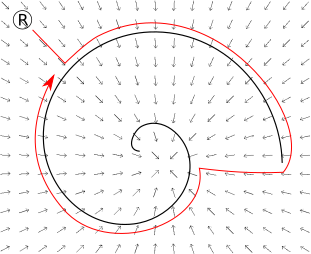
\includegraphics[width=\linewidth]{/home/ams/TinyRobo/docs/spiral_trap.png}
	\end{subfigure}
	\begin{subfigure}{0.45\textwidth}
		%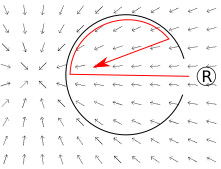
\includegraphics[width=\linewidth]{/home/ams/TinyRobo/docs/wall_follow_trap.png}
	\end{subfigure}
	\caption{Simple obstacles that result in looping behavior for a bug algorithm that combines wall following with leaving the obstacle when the vector field points away from the obstacle.}
	\label{traps_for_wall_follow}
\end{figure}

In none of these cases is the goal unreachable, in that it is a member of the same set of points as the open space of the environment, but attempts at obstacle avoidance preclude the robot reaching it. 

\section{Code Generation Refinement}

Rather than rejecting bug algorithms because they cannot be usefully combined with a global vector field, the vector field representation of the space was rejected. 
Vector fields have other problems, beyond unsatisfactory composition with complete motion control planners such as the bug algorithm family. 
A vector field cannot represent a path that crosses itself, such as a patrol route that is a loop.
In the continuous case, a vector field is represented by a function that maps all points in the space to a vector representing the desired robot heading at that point. 
However, because a function produces exactly one value, each point can only have one heading, while the intersection point of a path has two headings, at different points in time. 
For a vector field broken up into discrete grid cells, the same problem applies, but to regions rather than points. 

One potential solution to this problem with vector fields is to have multiple vector fields, or multiple values at each point, and allow the robot to maintain a program counter, which it uses to determine which field or which value to use at a given point. 
The counter is incremented on departure from a vector field grid cell, and then on return to that cell, the new value of the program counter is used in a guard, which results in the robot using the second value of the heading. 

For example, the GCPR statements:\\
(self.is\_in((1.745, 1.921), (1.245, 1.421)) and pc\_is(1), self.set\_desired\_heading(2.332), 0.9)\\
(self.is\_in((1.745, 1.921), (1.245, 1.421)) and pc\_is(2), self.set\_desired\_heading(1.031), 0.9)\\
will result in the robot using the heading 2.332 when it passes through the grid region if the program counter is 1, and 1.031 when it passes through the grid region with the program counter set to 2 (while, unfortunately, not defining a desired heading if the program counter is set to some other value).

Using a program counter to select possible headings for a discrete vector field grid cell has the drawback that the program counter must be incremented on leaving the cell, as incrementing it while remaining in the cell will cause a change of heading.
As a result, the generated program must have guards on all cells surrounding the cell, which increment the program counter when triggered. 

Further adding to this complexity is the problem of sensor noise. 
If sensor noise causes the robot to erroneously detect that it has entered the neighboring cell, then the program counter could be incremented without the robot actually leaving its current cell. 
On the next update of the noisy position sensor, the robot could then ``return'' to the current cell, and change direction due to the incorrectly implemented program counter. 

As a consequence of the complexity attendant on repairing the inability of the vector field to represent paths containing loops, the underlying representation of the conversion of user paths into robot programs was changed to avoid the use of vector fields. 

\subsection{Approaching a Point}

The basic action of the robot is to move from one location to another. 
Under the assumption that there exists some form of localization, which must hold in order to support the type of user interface described in this work, the simplest approach to navigation to a point is for the robot to rotate to face that point and then move forwards towards it. Once the point is reached, the robot should stop. 

Reaching of a point is more complex for swarm robots than it is for single robots. 
Some work assumes that robots in the abstract are points, and as they occupy no area, any number of them may congregate at a mathematical point. 
In the real world, while a point may be described precisely, it is usually sufficient to arrive within some small distance $\epsilon$ of it to say that the robot has reached the point. 
However, robots also take up space in the real world, and so as more and more members of the swarm arrive at the point, the later arrivals may be precluded from actually approaching to within $\epsilon$ of the point.
In this case, it is desirable to have a definition of arrival that expands to allow robots to approach the point as closely as they can and stop when that condition is met. 

For example, when a robot arrives at the point, it might stop, but broadcast a message to local robots that it is at the point. 
Robots arriving after the first would then navigate around it, keeping track of the minimum distance to the goal. 
After finishing a circumnavigation, the robot would then return to the closest point to the goal. 
As more robots arrive, the local minimum in the approach to the target point may become occupied by another robot, and so if that point is occupied, the robot would then have to perform another circumnavigation to find a new closest point. 
Because every iteration of this loop either occupies the closest point with a robot, or detects that the closest point has become occupied by another robot, and triggers another iteration, it will eventually position every robot as close as possible to the goal. 

\section{Completeness of Navigation}

Moving to a point is implemented as a bug algorithm. As described earlier, bug algorithms are complete, in that they navigate the robot to a point, or determine that the point cannot be reached. A review of eleven bug algorithms can be found in \citep{ng2007performance}. 

As stated earlier, it is preferable to have the robots follow the user-specified path, as following the user path is both more understandable to the user, and may allow the system to use information that the user has and the robot does not. 
A user path can be followed by a bug algorithm by breaking the user path into a series of points, and using a bug algorithm to navigate to each point in turn. 
Because the bug algorithm is complete, it can either reach the target point, or determine in finite time that the point is not reachable. 
For every point except the last in the user path, if the point is not reachable, the program can simply reset its target point to the next point along the path. 
Dropping points from consideration in this way will result in the robot deviating from the path, but the reason for the deviation is clearly explainable to the user, both from a program logic standpoint, and visually, as the interface displays the progress of the robot around the obstacle. 
If the last point of the user path is not reachable, the user-commanded path cannot be successfully completed, and so the user should be informed that the robot cannot reach it. 

Unfortunately, most of the bug algorithms have the requirement that the obstacles in the environment are not moving.
Indeed, the presence of moving obstacles results in navigation becoming undecidable without knowledge of the future movement of the obstacles, as an obstacle can move to occupy the robot's goal. 
Unless it is known whether the obstacle will move off the goal in the future, it cannot be determined whether the goal is unreachable, or just not currently reachable. 

The Tangent-bug algorithm has been extended to handle moving obstacles, given a number of constraints \citep{kamon1998tangentbug, tomita2009sensor}.
The main constraint that affects the use of this algorithm is that the obstacles are constrained to be moving at a velocity that is slower than that of the robot.
This constraint is required because if the robot is circumnavigating the obstacle, and the obstacle is moving faster than the robot, then in the time that the robot requires to circumnavigate the perimeter of the obstacle, the obstacle will have moved a distance greater than its own perimeter is long, and the circumnavigating robot will have moved with it.
As a consequence, the circumnavigating robot might not return to its own previous path and cross it, which is the condition that Tomita and Yamamoto use to determine that the robot should leave the obstacle. 

At first, this would appear to be a problem for swarm robots, because if the robots are the same, they will be moving at the same speed. 
If one moves in a straight line, and the other attempts to circumnavigate it, the circumnavigating robot will never cross its own path for the reason described above, and so never leave. 
However, if the robots are using the same bug algorithm, this trap will not be sprung, because each robot will attempt to circumnavigate the other. 
If they attempt to circumnavigate each other in opposite directions, they will spiral around each other, leading to at least one of the robots crossing its own previous path, and triggering the leave condition of the algorithm. 
If they attempt to circumnavigate each other in the same direction, they will come to a position side-by-side, as neither can outpace the other, but neither will pull away from the other because they are attempting to follow each other's perimeters. 
In this case, they are pointed towards the goal, because in the absence of an obstacle, Tomita and Yamamoto's modified Tangent-bug orients the robot towards the goal, and so before they encountered each other, the robots were oriented towards the goal.
The robots will then approach the goal, and one will arrive, while the other circumnavigates the first until it detects that it cannot arrive at the goal. 

Tomita and Yamamoto do not deal with the decidability of their modification of Tangent-bug because they constrain the goal point to be not within an obstacle, and so reachable by the robot. The original Tangent-bug will navigate the robot to the goal if it is reachable, or circumnavigate the obstacle, returning to its starting point, whereupon it detects that the point is unreachable \citep{kamon1998tangentbug}. Since Tomita and Yamamoto constrain the goal to not be within an obstacle, the original Tangent-bug will reach it. 

In the case of moving obstacles, if the goal is covered by an obstacle, the obstacle is either moving or not moving. If the obstacle is moving, the modified Tangent-bug will not return to its original hit point, which is either left behind or covered by the obstacle, but will eventually cross itself, and leave the object towards the goal.
If the obstacle is still covering the goal, this process will repeat until the object is not covering the goal anymore, and the robot will reach the goal. 

In the case of swarm robots, as described above, some mechanism may be needed to determine that the goal is occupied, possibly by other swarm members, and to stop at a location near the goal. 
The stopping condition of the original Tangent-bug in the case where the goal is unreachable extends naturally to swarm robots. 

If a robot is the first to arrive at the goal, the goal is not occupied, so the robot occupies it and stops. 
If a robot is not first to arrive at the goal, the goal is occupied by a robot, which is stopped. 
The new arrival treats the stopped robot as an obstacle, circumnavigates it, returns to the original hit point and so detects that the goal is unreachable, and stops. 
If multiple new arrivals get to the stopped robot(s) at the same time, the conditions above hold, and so they eventually either cross their own paths while trying to circumnavigate another robot that is also circumnavigating an obstacle, and so leave and return (and so become later arrivals), or complete a circumnavigation and return to their own starting point and stop (becoming part of the obstacle).

If a maximally dense cluster of robots is desired, the unreachability check of Tangent-bug can be extended. 
Once the goal is determined to be unreachable, the robot performs another circumnavigation of the blocking obstacle to find the closest point to the goal, and returns to that point. 
That point has either been occupied by another robot, in which case the robot repeats this step, or occupies that point if it is free. 
Because every iteration of this step fills the point closest to the goal with a robot, the cluster of robots is packed as close to the goal as possible. 

 \begin{figure}
 	\centering
 	\digraph[scale=0.6]{TangentBugMod}{
 		
 		start -> obstacleToGoal;
 		obstacleToGoal -> aimToGoal [label="No"];
 		aimToGoal -> atGoal;
 		atGoal -> stop [label="Yes"]; 
 		atGoal -> obstacleToGoal [label="No"];
 		obstacleToGoal -> recordHit  [label="Yes"];
 		recordHit -> followEdge;
 		followEdge -> closerPoint;
 		closerPoint -> leaveObstacle [label="Yes"];
 		leaveObstacle -> obstacleToGoal;
 		closerPoint -> pathCross [label="No"];
 		pathCross -> returnToHit [label="No", color="blue"];
 		returnToHit -> followEdge [label="No", color="blue"];
 		returnToHit -> unreachable [label="Yes", color="blue"];
 		unreachable -> lastPoint [color="blue"];
 		lastPoint -> updateGoal  [label="No", color="blue"];
 		lastPoint -> stop  [label="Yes", color="blue"];
 		updateGoal -> obstacleToGoal [color="blue"];
 		pathCross -> obstacleToGoal3 [label="Yes"];		
		obstacleToGoal3 -> followEdge2 [label="Yes"];		
		obstacleToGoal3 -> aimToGoal[label="No"];		
		followEdge2 -> obstacleToGoal3;
		
 		obstacleToGoal [label="Obstacle in direction of goal?"];
 		aimToGoal [label="Orient towards and move to goal"];
 		atGoal [label="At goal?"];
 		leaveObstacle[label="Leave obstacle"];
 		recordHit [label="Record hit point"];
 		unreachable [label="Goal is unreachable", color="blue"];
 		updateGoal [label="Next point is new goal", color="blue"];
 		lastPoint [label="Is this the last point?", color="blue"];
 		followEdge [label="Follow obstacle edge"];
 		returnToHit [label="Returned to hit point?", color="blue"];
 		closerPoint [label="Closer to goal than hit point?"];
 		pathCross [label="Crossed own path?"];
 		obstacleToGoal3 [label="Obstacle in direction of goal?"];
 		followEdge2 [label="Follow obstacle edge"];
 	}
 	\caption{The proposed modifications (in blue) to the Tomita and Yamamoto Tangent-bug algorithm for user path following in cases with multiple robots, some of which may be treated as moving obstacles. This flow chart does not include the option for maximally dense packing at the goal described in the text. }
 \end{figure}

\chapter{Compiler Verification}

The design of a compiler which verifies that its output is correct What does it mean for a program to be correct? Free from things like assignment of variables to the wrong type, buffer overflows, off-by-one errors, etc. Does not mean that the program does what the programmer intended, just that it does whatever it does without errors. 
Correctness is judged with respect to a specification. 
Partial correctness - if an answer is returned, it is correct. 
Total correctness - requires that program is partially correct and terminates
No general solution to halting problem, needs specific proof per-program
Compiler correctness shows that a compiler behaves according to its specification
I don't currently have a language specification for the gesture language 

One method of testing compilers is the operation of a fuzzer \citep{miller1990empirical}. A fuzzer, in the general case, generates input for programs that, while technically legitimate input, causes unexpected behavior such as program crashes. A fuzzer for compilers uses a description of the source language to generate programs that are considered valid under the description, and then attempts to compile them using the compiler. It can also attempt to generate programs that are deliberately incorrect, to test the ability of the compiler to accurately report errors, and to ensure that the compiler accepts all correct programs and no incorrect programs, as in \citep{bazzichi1982automatic}. 
Because the internal structure of the compiler is not known, a generator cannot be certain that it causes all code paths in the compiler to be executed, but it can be certain that the generated test programs use all of the syntactical elements of the language, since all of the elements are described in the language specification. Interestingly, Bazzichi and Spadafora's work predates the use of the term ``fuzzer'' by 8 years, but clearly describes the same process.

Translation validation \citep{pnueli1998translation}
verifies compiled code against input code rather than attempting to verify that a compiler correctly translates all input programs.
Verifies that the compiler correctly transforms a specific input program. 
Needs:
 - A common semantic framework for the representation of the source code and the generated target code (probablistic finite automaton?)
 - A formal description of "correct implementation"
 - A proof method for verifying that one instance of the semantic framework (the output) correctly implements another one (the input)
How is the IR not the common semantic framework?
%
 


